\hypertarget{tablica_8cpp}{\section{Dokumentacja pliku prj/tablica.cpp}
\label{tablica_8cpp}\index{prj/tablica.\-cpp@{prj/tablica.\-cpp}}
}


Definicja metody Dodaj\-Na\-Koniec.  


{\ttfamily \#include \char`\"{}tablica.\-hpp\char`\"{}}\\*
{\ttfamily \#include $<$fstream$>$}\\*
Wykres zależności załączania dla tablica.\-cpp\-:
\nopagebreak
\begin{figure}[H]
\begin{center}
\leavevmode
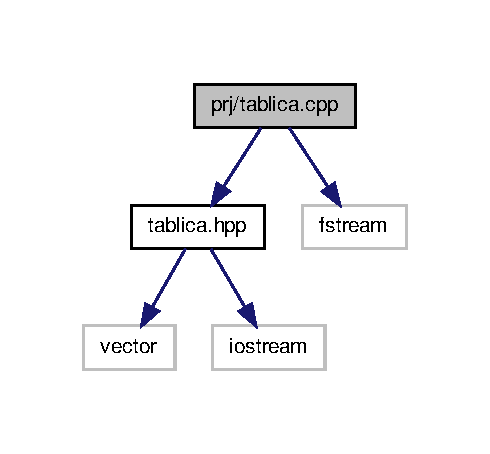
\includegraphics[width=235pt]{tablica_8cpp__incl}
\end{center}
\end{figure}


\subsection{Opis szczegółowy}
Definicja metody Dodaj\-Na\-Koniec. Definicja przeladowania operatora == .

Definicja przeladowania operatora = .

Definicja przeladowania operatora + .

Definicja metody Usun\-Ele.

Definicja metody Wyswietl\-Tab.

Definicja metody Pobierz\-Wskazany\-Ele.

Definicja metody Dodaj\-Na\-Miejsce.

Definicja metody Odwroc\-Tab.

Definicja metody zamien elementy.

Definicja metody Pobierz\-Rozmiar.

Definicja metody Pobierz\-Ostatni\-Ele.

Definicja metody Pobierz\-Pierwszy\-Ele.

Definicja metody Dodaj\-Na\-Poczatek.

Metoda, ktora dodaje na koniec element.

Metoda, ktora dodaje na poczatek element.

Metoda, ktora pobiera pierwszy element.

Metoda, ktora pobiera ostatni element.

Metoda, ktora pobiera pobiera rozmiar tablicy.

Metoda, ktora zamienia dwa wybrane elementy.

Metoda, ktora odwraca tablice.

Metoda, ktora dodaje element na konretne miejsce.

Metoda, ktora pobiera wskazany element.

Metoda, ktora wyswietla tabilce.

Metoda, ktora dusuwa elementy.

W celu lacznia dwoch tablic w jedna.

W celu przypisania dwoch tablic.

W celu lacznia porownania tablic. 

Definicja w pliku \hyperlink{tablica_8cpp_source}{tablica.\-cpp}.

